\documentclass[11pt, oneside]{article}

\usepackage[english]{babel}
\usepackage{geometry}
\usepackage{graphicx}
\usepackage{tabularx}
\usepackage{amssymb}
\usepackage{amsmath}
\usepackage{booktabs}
\usepackage{xltabular}
\usepackage[hyphens]{url}
\usepackage{hyperref}
\hypersetup{breaklinks=true,hidelinks}
\usepackage[backend=bibtex,style=nature]{biblatex}
\addbibresource{references.bib}

\usepackage{csquotes}
\usepackage{cleveref}
\usepackage{siunitx}
\usepackage{geometry}
\usepackage{multirow}
\geometry{left=4.2cm, right=4.2cm}

\usepackage[dvipsnames]{xcolor}
\definecolor{tumblue}{rgb}{0,0.396078431372549,0.741176470588235}

\usepackage{xspace}
\usepackage{caption}
\usepackage{subcaption}
\usepackage{authblk}
\usepackage{mhchem}


\usepackage{marvosym}

\usepackage{sectsty}

%\usepackage[sort&compress,numbers,super]{natbib}

\sectionfont{\color{tumblue}\selectfont\sffamily}
\subsectionfont{\color{tumblue}\selectfont\sffamily}
\subsubsectionfont{\color{tumblue}\selectfont\sffamily}
\paragraphfont{\selectfont\sffamily}
\subparagraphfont{\color{gray}\selectfont\sffamily}


\renewcommand*{\Authfont}{\sf}
\renewcommand*{\Affilfont}{\sf}


\definecolor{halfgray}{gray}{0.55}
\renewcommand\labelitemi{\color{halfgray}$\bullet$}
%\usepackage{kpfonts}


\clubpenalty = 10000
\widowpenalty = 10000
\displaywidowpenalty = 10000


% if the \fonts folder exists, use fontspec to change fonts
\IfFileExists{./fonts/Heliotrope-Bold.otf}{
    \usepackage{fontspec}
    \setmainfont{Heliotrope}[Extension = .otf, UprightFont = *-Regular, ItalicFont = *-Italic, BoldFont=*-Bold, Path = ./fonts/]
}{
    \usepackage{biolinum}
    \renewcommand{\familydefault}{\sfdefault}
}

\makeatletter
\renewbibmacro*{textcite}{%
  \iffieldequals{namehash}{\cbx@lasthash}
    {\usebibmacro{cite:comp}}
    {\usebibmacro{cite:dump}%
     \ifbool{cbx:parens}
       {\bibclosebracket\global\boolfalse{cbx:parens}}
       {}%
     \iffirstcitekey
       {}
       {\textcitedelim}%
     \usebibmacro{cite:init}%
     \ifnameundef{labelname}
       {\printfield[citetitle]{labeltitle}}
       {\printnames{labelname}}%
     \addspace
     \ifnumequal{\value{citecount}}{1}
       {\usebibmacro{prenote}}
       {}%
     \mkbibsuperscript{\usebibmacro{cite:comp}}%
     \stepcounter{textcitecount}%
     \savefield{namehash}{\cbx@lasthash}}}
\makeatother


\usepackage{lipsum}
\usepackage[labelfont=bf]{caption}

\renewcommand{\Affilfont}{\scriptsize}
 \renewcommand{\Authfont}{\normalsize}

 \usepackage{microtype}


\clubpenalty = 10000
\widowpenalty = 10000
\displaywidowpenalty = 10000

\errorcontextlines=10


\usepackage{tikz}
 \usetikzlibrary{positioning,fit,backgrounds,arrows.meta,calc}
\usepackage{xcolor}


\definecolor{dangercolor}{RGB}{180,30,30} % not used strongly; kept for compatibility
\definecolor{chemcolor}{gray}{0.2}        % not used strongly; kept for compatibility
\definecolor{metacolor}{gray}{0.2}        % not used strongly; kept for compatibility


\usepackage{credits}
\usepackage{orcidlink}
\usepackage{showyourwork}

\title{\textsf{Clever Materials: When Machine Learning Models Fool Themselves}}

\author[1,2, 3, 4, \Letter]{Kevin~Maik~Jablonka~\orcidlink{0000-0003-4894-4660}}



\affil[1]{Laboratory of Organic and Macromolecular Chemistry (IOMC), Friedrich Schiller University Jena, Humboldtstrasse 10, 07743 Jena, Germany}
\affil[2]{Helmholtz Institute for Polymers in Energy Applications Jena (HIPOLE Jena), Lessingstrasse 12-14, 07743 Jena, Germany}
\affil[3]{Center for Energy and Environmental Chemistry Jena (CEEC Jena), Friedrich Schiller University Jena, Philosophenweg 7a, 07743 Jena, Germany}
\affil[4]{Jena Center for Soft Matter (JCSM), Friedrich Schiller University Jena, Philosophenweg 7, 07743 Jena, Germany}



\affil[\Letter]{\texttt{mail@kjablonka.com}}


\begin{document}

\maketitle

\begin{abstract}
	...
\end{abstract}

\section{Introduction}

Learning from data is appealing but also scary. 
It is appealing because it promises to make predictions that are too subtle or complex for humans to recognize.\autocite{hardtrecht2022patterns} 
It is scary because some of these patterns might be meaningless and thus lead to complete failures of predictions.\autocite{Lones2024}

Exploiting meaningless patterns --- which can lead to impressive performance in demonstrations but complete failures in other tests --- is a known failure mode of pattern recognition. 
It is often discussed in the context of the horse \enquote{Clever Hans}.\autocite{Lapuschkin2019} 
The horse \enquote{Clever Hans} was thought to be able to count. This was until it was found that \enquote{Clever Hans} could not count but rather relied on subtle clues from his owner in creating the answer. 

In image recognition models, this Clever Hans effect has been demonstrated in breadth. Models rely on spurious correlations (also called \enquote{shortcuts})\autocite{Brown2023, Howard2021} --- skin color on clinical images,\autocite{pooch2019trust} or the background on images of animals,\autocites{xiao2020noise}. 
Recently, the startup Leash Biosciences reported that such failure modes might also hamper bioactivity predictions.\autocite{leash} 
Models are surprisingly good at predicting who produced a compound. 
This is an intent signal that models might exploit in making activity predictions. 

This seems like a reasonable, but also worrying, failure mode. 
Also in other chemical and material domains one might expect a lot of potential for proxy signals a model could exploit that are not directly linked to any (causal) understanding of chemistry: We know that certain groups focus on optimizing stability of solar cells, the university or research group name is sometimes even part of the name of a metal-organic framework --- and we know the research agendas of different groups (\Cref{fig:clever_hans}). 
Similarly, we know that research fields evolve and performance tends to grow with discoveries of certain materials design features:\autocite{shabih2026autonomous} Be it self-assembled monolayers in perovskite solar cells or post-synthetic modification in MOFs.

\begin{figure}
	\centering 
	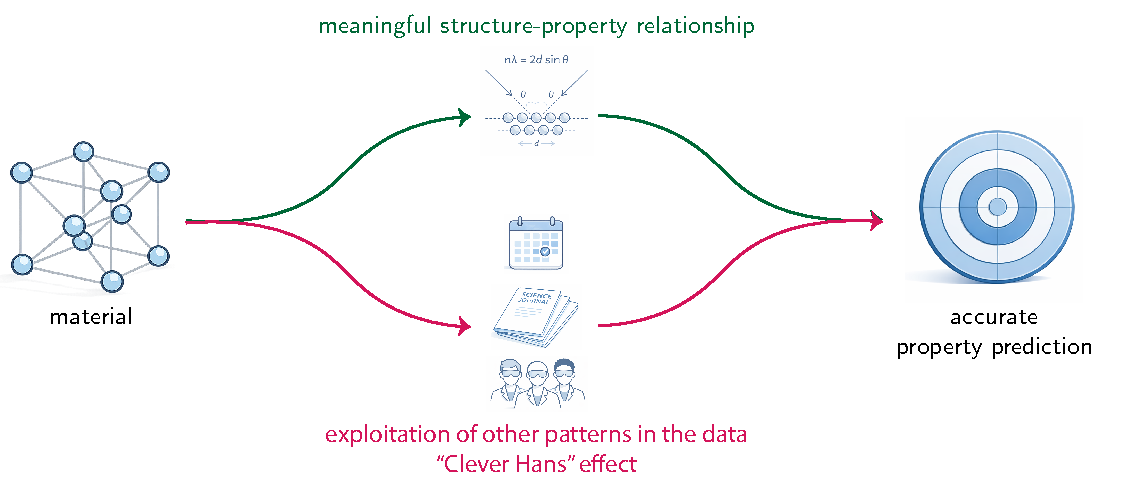
\includegraphics[width=\textwidth]{../static/clever_materials_hans_overview.pdf}
	\caption{\textbf{In machine learning, we often do not test competing hypotheses of how a model might obtain its answers.} Machine learning models in materials science are trained to map material (descriptors) to property predictions. Models have much flexibility in how they learn this map from data. Ideally, they discover robust and meaningful structure-property relationships that also generalize in new settings. This, however, is not guaranteed. Models might also exploit other patterns in the data as a shortcut to a prediction (\enquote{purple}). For instance, it might be easy for the model to spot what researchers produced a given material or in what journal it has been published. Based on those inferences, it might deduce property \enquote{guesses} (as the knowledge of the research group or the publication time can be correlated to the property). The model thus might learn to make good predictions for the wrong reasons. This is known as the \enquote{Clever Hans} effect. The scientific method asks us to test if such alternative patterns can explain good model performance. This is seldom done. In this work, I do it for a few case studies. }	
	\label{fig:clever_hans}
\end{figure}


In this work, I investigate how relevant such confounders are in commonly used materials datasets. For this, I enrich datasets that have been used for material property prediction tasks with meta information such as author names, publication years, or publication venue.
I show that this metainformation can often be predicted with surprising accuracy. Models trained on those predicted \enquote{metainformation fingerprints} show, in some cases, performance that is indistinguishable from models that are trained on \enquote{meaningful} descriptors. 

These findings underline --- again --- how easy it is to fool oneself in machine learning (in the chemical sciences). But they also provide indications on how to improve data collection efforts and improve the validation of scientific machine learning models. 
  


\section{Results}

I analyzed how severe the Clever Hans problem might be across five different materials case studies spanning organic electronics, energy storage, and porous materials. Since results depend not only on the dataset but also on the prediction task and the metrics one uses to analyze the results, I report additional variants of some of the case studies in the appendix.
The code is reusable and can be easily applied to other case studies. 

\subsection{MOF Thermal Stability}

Metal-organic frameworks (MOF) are being trialed for various applications.\autocite{Kalmutzki2018} 
In many of those applications, thermal stability is an essential criterion. 
To be able to model this, \textcite{Nandy2022} mined thermogravimetric analysis data from the literature and derived decomposition temperatures. 
Based on this, one can build models to predict the decomposition temperature (a regression problem)\autocite{Nandy2021} or whether a given structure belongs to the most stable ones (a binary classification problem).
\Cref{fig:mof_thermal_stability} shows how well one can predict meta-information based on materials descriptors and, based on those predictions, whether the MOF belongs to the top 10\% most stable ones.

\begin{figure}
	\centering 
	\caption{\textbf{For the classification task of membership in the top-10\% of thermally stable MOFs, one can be fooled (by Clever Hans effects).} The model can predict the bibliographic information with high accuracy. \textbf{a} The model predicts the authors of the associated paper with high accuracy, much better than a random baseline. \textbf{b} This also holds for predicting in which journal the entry was published or the year in which the paper was published (\textbf{c}). Using the predicted bibliographic information, a model can also predict with high accuracy if the MOF belongs to the top-10\% thermally stable ones. However, one needs to highlight that the effect is smaller --- or not even there --- if analyzed under a different metric or for a regression setting. The dummy baseline for classification is a stratified random sampling (using the empirical probabilities from the training dataset) and the mean prediction for the regression case.}
	\label{fig:mof_thermal_stability}	
\end{figure}




\subsection{MOF Solvent Stability}

Besides thermal stability, solvent stability is an essential requirement for MOF application. Solvent stability describes whether a structure collapses when bound solvent (e.g., from the synthesis) is removed under activation (e.g., using vacuum and heat). This data, too, was text-mined by \textcite{Nandy2022} and I used the same descriptors. And for this property, too, \textcite{Nandy2021} reported machine learning models. As for the thermal stability case study, I use similar features in my model.

\begin{figure}
	\centering 
	\caption{}
	\label{fig:mof_solvent_stability}
\end{figure}

\Cref{fig:mof_solvent_stability} shows that for this case, too, materials descriptors can predict bibliographic information with high accuracy. While the model trained to directly map material descriptors to solvent stability outperforms the one where we use the predicted bibliographic information to predict solvent stability, this \enquote{Clever Hans} model still meaningfully outperforms the baseline.


\subsection{Perovskite Solar Cell Efficiency}

Perovskite solar cells are another way in which materials scientists aim to have a positive impact on the energy transition.\autocite{CorreaBaena2017}
A metric of central importance here is the power conversion efficiency (PCE). 
It was mined by \textcite{Jacobsson2021} in a manual approach and by \textcite{shabih2026autonomous} in an automated one with large language model-based data extraction.\autocite{SchillingWilhelmi2025} 


\begin{figure}
	\centering 
	\caption{}
	\label{fig:perovskite_pce_classification}
\end{figure}

As a case study, I again analyze whether we can predict whether the device belongs to the top 10\% efficient devices. For both the \enquote{Conventional} and \enquote{Clever Hans} models, I derive descriptors for the composition of the absorber. 



\subsection{Battery Capacity}

For sustainability, energy does not only need to be converted. For this, batteries are important. \textcite{Huang2020} text-mined battery materials alongside performance metrics. 

\begin{figure}
	\centering 
	\caption{Battery capacity}
	\label{fig:battery_capacity}
\end{figure}

\Cref{fig:battery_capacity} shows that while the model can predict bibliographic information better than the random baseline based on the composition features, it still does so with relatively low performance.
The prediction of the publication year shows higher performance.


\subsection{TADF Emitter Properties}

Thermally activated delayed fluorescence (TADF) is one mechanism to improve the efficiency of organic light-emitting diodes (OLED)s.\autocite{Liu2018} The maximum emission wavelength is one important performance metric that is optimized for these materials. \textcite{Huang2024} text-mined using ChemDataExtractor.\autocite{Swain2016, Mavrai2021}

As a feature set for the \enquote{Conventional} and \enquote{Clever Hans} models, I use a broad set of molecular descriptors and fingerprints. Both \enquote{Conventional} and \enquote{Clever Hans} models aim to predict the maximum emission wavelength. 

\section{Discussion}

Machine learning has transformed materials discovery,\autocite{Moosavi2020, Saal2020, Gubernatis2018} but the findings here highlight a critical gap: we often fail to rigorously test alternative hypotheses for why our models perform well. 
The scientific method demands that we actively seek to falsify our hypotheses,\autocite{Platt1964, popper2005logic, Chamberlin1965} yet in machine learning, we tend to focus on optimizing performance rather than exploring competing explanations.

The Clever Hans effect represents just one class of alternative hypotheses we should systematically explore. 
When we claim that models \enquote{learn meaningful chemistry,} we must test whether simpler explanations --- such as author identity or temporal trends --- could account for the observed performance.\autocite{Chuang2018} 
This requires a shift from asking \enquote{does this model work?} to \enquote{why does this model work, and what are all the ways it could be wrong?}

The space of potential confounders is vast and often non-obvious. Beyond meta-information, models might exploit dataset construction artifacts, measurement biases, or subtle correlations we have not considered. 
Systematically exploring these alternatives is computationally intensive but crucial for scientific rigor.

LLM-based agents might offer a promising approach to automate this exploration.\autocite{Ramos2025, alampara2025general} 
These systems could generate and test competing hypotheses in parallel, exploring the space of potential explanations more thoroughly than human researchers typically manage. 
Such agents could serve as \enquote{devil's advocates,} systematically challenging our assumptions about why models succeed.

\subsection{Toward Robust Materials Data Infrastructure}

Another angle is to reconsider how we generate, curate, and share materials data. 
The field needs coordinated infrastructure that prioritizes diversity and robustness over convenience. \autocite{Krishnan2025}
Convenience and short-term reward are often too easy and compelling to optimize for due to collective action problems trapping an ecosystem in a suboptimal state, where every actor knows that changes would be needed, but no one wants to make the first move.\autocite{Nielsen2020-rr} 

The most obvious issue is data generation itself. Most automated screening approaches optimize specific objectives using limited building blocks, which creates exactly the kind of proxy signals that models learn to exploit. 
What we need are organizations that can generate diverse data at scale---potentially focused on the lowest cost per reproducible data point rather than pushing particular research agendas.

Perhaps most importantly, we need to change how we evaluate models. 
Instead of asking whether models work, we should ask why they work and systematically explore alternative explanations. 
This means actively trying to disprove our own --- but also others' --- claims about model performance.
To enable others to do so, access to data and code is obviously a prerequisite. But one could also envision that some of these tests might require new experiments --- which could be facilitated using infrastructure as a service or incentivized using \enquote{bug bounties} for research papers, models, or datasets. We need to accept that receiving feedback --- even if it is pointing out a mistake in our own work --- is a gift.

\section{Conclusions}

Model evaluation has always been challenging in materials science.\autocite{Alampara2025} 
We have developed increasingly sophisticated techniques to address this: time-based splitting,\autocite{sheridan2013time, Landrum2023} scaffold splits, leave-one-cluster-out cross-validation,\autocite{Durdy2022, Meredig2018} cluster-based splits,\autocite{guo2024scaffold} and property-based splits.\autocite{Jablonka2023, kunchapu2025polymetrix} Each technique revealed new ways that models could fail to generalize, forcing us to be more rigorous in our evaluation practices.

This work highlights yet another layer of complexity. Models can achieve impressive performance not by learning meaningful chemistry, but by exploiting subtle biases in how our datasets are constructed. Across five different materials domains, I find that proxy signals based on publication meta-information consistently provide substantial predictive power.

The simplest explanation for good model performance is often shortcut learning, not meaningful chemistry. This is an uncomfortable truth that challenges fundamental assumptions about what our models learn. The space of potential confounders extends far beyond what current evaluation techniques can catch.

Like the original Clever Hans, our models may be performing impressive feats---but for all the wrong reasons. They excel not because they understand chemistry, but because they have learned to read the subtle cues we inadvertently embedded in our data. The question is no longer whether our models can achieve good performance, but whether we can trust what that performance actually means.

This is not necessarily a condemnation of all shortcut learning. Models that exploit proxy signals can still provide statistically reliable predictions and practical value---as long as the underlying patterns remain stable. The critical issue is transparency about what we are doing and why.

If our goal is scientific understanding and robust generalization to genuinely new materials, we must systematically explore alternative explanations and build models that resist spurious correlations. If our goal is simply a predictive tool that works well on average, we can accept some brittleness---but we should communicate openly that the model may fail in unpredictable ways when the hidden assumptions break down.

In the end, the Clever Hans problem forces us to confront a choice about scientific machine learning: Do we want tools that advance chemical understanding, or are we content with sophisticated pattern matchers that reflect our own biases? Both approaches have merit, but honesty about which path we are taking will help to unlock real acceleration using machine learning. 

\section{Methods}

\subsection{Clever Hans Analysis Framework}

I implemented a systematic framework to quantify Clever Hans effects in materials property prediction. For each dataset, I trained three types of models: (1) conventional models that predict material properties directly from chemical descriptors, (2) indirect models that first predict meta-information (author identity, journal, publication year) from the same descriptors and then use these predictions to estimate material properties, and (3) dummy baselines using stratified sampling for classification or mean prediction for regression.

The indirect prediction approach tests whether meta-information contains sufficient signal to achieve competitive prediction performance. If models can predict material properties as accurately using only proxy information as using chemical descriptors, this indicates potential Clever Hans effects in the dataset.

\subsection{Model Architecture and Training}

All models used gradient boosting, implemented with \texttt{LightGBM}\autocite{lightgbm} with default hyperparameters. I performed 10-fold cross-validation with random shuffling for all analyses. Each fold compared performance across the three model types using identical train/test splits to ensure paired comparisons.


\subsection{Datasets and Feature Engineering}

\subsubsection{Battery Dataset}
I obtained the battery dataset from \textcite{Huang2020}

%The battery dataset contained \input{output/battery_dataset_size} entries with \input{output/battery_n_features} chemical descriptors.
%[To be filled: Describe the specific chemical descriptors used for battery capacity prediction]
%
\subsubsection{Perovskite Dataset} 
I obtained the perovskite dataset from \textcite{shabih2026autonomous}, which is based on \textcite{Jacobsson2021}.

%The perovskite dataset contained \input{output/perovskite_dataset_size} entries with \input{output/perovskite_n_features} descriptors.
%[To be filled: Describe the descriptors used for perovskite solar cell efficiency prediction]
%
\subsubsection{MOF Datasets}
I obtained the MOF datasets from \textcite{Nandy2022}. The dataset already contains precomputed features such as  revised autocorrelation functions.\autocite{Moosavi2020} 

%The MOF thermal stability dataset contained \input{output/mof_thermal_dataset_size} entries with \input{output/mof_thermal_n_features} structural and chemical descriptors. The MOF solvent stability dataset contained \input{output/mof_solvent_dataset_size} entries with \input{output/mof_solvent_n_features} descriptors.
%[To be filled: Describe the structural and chemical descriptors used for MOF thermal stability and solvent stability prediction]
%
\subsubsection{TADF Dataset}
I obtained the TADF dataset from \textcite{Huang2024}. 
%The TADF dataset contained \input{output/tadf_dataset_size} entries with \input{output/tadf_n_features} molecular descriptors.
%[To be filled: Describe the molecular descriptors used for TADF property prediction]

\subsection{Chemical Descriptor Generation}

For datasets containing molecular or compositional information, I generated comprehensive chemical descriptors to serve as baseline features for property prediction. 

\subsubsection{Molecular Descriptors from SMILES}
For datasets with SMILES (Simplified Molecular-Input Line-Entry System) strings,\autocite{Weininger1988} I computed molecular descriptors using RDKit \autocite{rdkit}. The molecular feature set included:

\begin{itemize}
    \item \textbf{2D descriptors}: All available RDKit molecular descriptors ($\sim$200 features), including molecular weight, LogP, topological polar surface area, number of aromatic rings, hydrogen bond donors/acceptors, and rotatable bonds.
    \item \textbf{Fingerprints}: 2048-bit circular fingerprints with radius 2, capturing local chemical environments and structural motifs.
\end{itemize}

Molecules were parsed from SMILES strings, and invalid or unparseable structures were excluded. 
\subsubsection{Composition Descriptors}
For datasets with chemical formulas (battery materials, perovskites), I computed composition-based descriptors using matminer \autocite{matminer}. The composition feature set included:

\begin{itemize}
    \item \textbf{Element properties}: Elemental statistics (mean, standard deviation, range) for atomic properties including atomic radius, electronegativity, ionization energy, and electron affinity using the Magpie preset \autocite{ward2016general}.
    \item \textbf{Stoichiometric features}: Composition statistics including element fractions, number of components, and chemical complexity metrics.
    \item \textbf{Meredig descriptors}: Extended element property statistics including orbital contributions and chemical bonding characteristics \autocite{meredig2014combinatorial}.
\end{itemize}

Chemical formulas were parsed using pymatgen \autocite{pymatgen}, and compositions that could not be parsed were excluded from analysis. 

\subsubsection{Feature Processing}
Generated descriptors were processed to handle missing values and ensure numerical stability for gradient boosting models. Features with excessive missing values ($>$50\%) were excluded, and remaining missing values were imputed with feature medians. For XGBoost and LightGBM models, additional preprocessing included clipping extreme values to prevent numerical overflow and replacing infinite values with conservative bounds.

\subsection{Meta-Information Extraction}

I enriched the datasets with publication meta-information using the Crossref API to retrieve bibliographic data, including author names, journal titles, and publication years. I created binary features indicating the presence of the top-$N$ most frequent authors and journals in each dataset, where $N$ was varied across 10, 50, 100, and 500 (or maximum available).

\subsection{Data Processing}

All datasets were preprocessed to remove entries with missing target values or author information. 


\subsection*{Data Availability}

The datasets used in this study are available on Zenodo: [DOI placeholder].

\subsection*{Code Availability}

All analysis code is available on GitHub: [URL placeholder].

\section*{Acknowledgement}
This work was supported by the Carl Zeiss Stiftung. The author is member of the NFDI consortium FAIRmat - Deutsche Forschungsgemeinschaft (DFG) - Project 460197019.

\section*{Declaration of Generative AI and AI-assisted Technologies in the Research and Writing Process}
I used Anthropic's Claude models as \enquote{copilot} in code development. I also used those models to improve language and readability. After using this service, I reviewed and edited the content as needed and take full responsibility for the content of the publication.

\printbibliography

\pagebreak

\appendix

\section{Detailed Results}
In this section, I show performance for metadata and property prediction in more detail. 


\end{document}
